This chapter intends to implement and analyse a controller ensuring safety if the demands from \autoref{def:cbf} %{req1}, \ref{req2} and \ref{req3} 
are obeyed. This shall first be tested on the slide movement on the da Vinci surgical robot as it comprises a prismatic joint and a 1:1 mapping from slide $joint\_angle$ to 1D position. Hence any inverse kinematics solver can be bypassed in the early phase of this project which is an important simplification to eliminate initial complications.

The slide movement is visualized in \autoref{fig:slidefig} and an overview of terms used in this section is found in \autoref{fig:safe:overview}, which also encompasses  the case study considered in this chapter. It puts forth the demands that the upper slide region, i.e. the interval $[\Lambda_{h+},\Lambda_\text{lim+}]$ is an unsafe area and the rest is considered safe. Furthermore, everything outside the slide physical limits, i.e. $[-\infty,\Lambda_\text{lim-}]$ and $[\Lambda_\text{lim+},\infty]$ is also considered unsafe. This case study is purely made up with the purpose to demonstrate the use of a safety controller.
\begin{figure}[H]
\centering
\subbottom[Illustration of slide movement.]{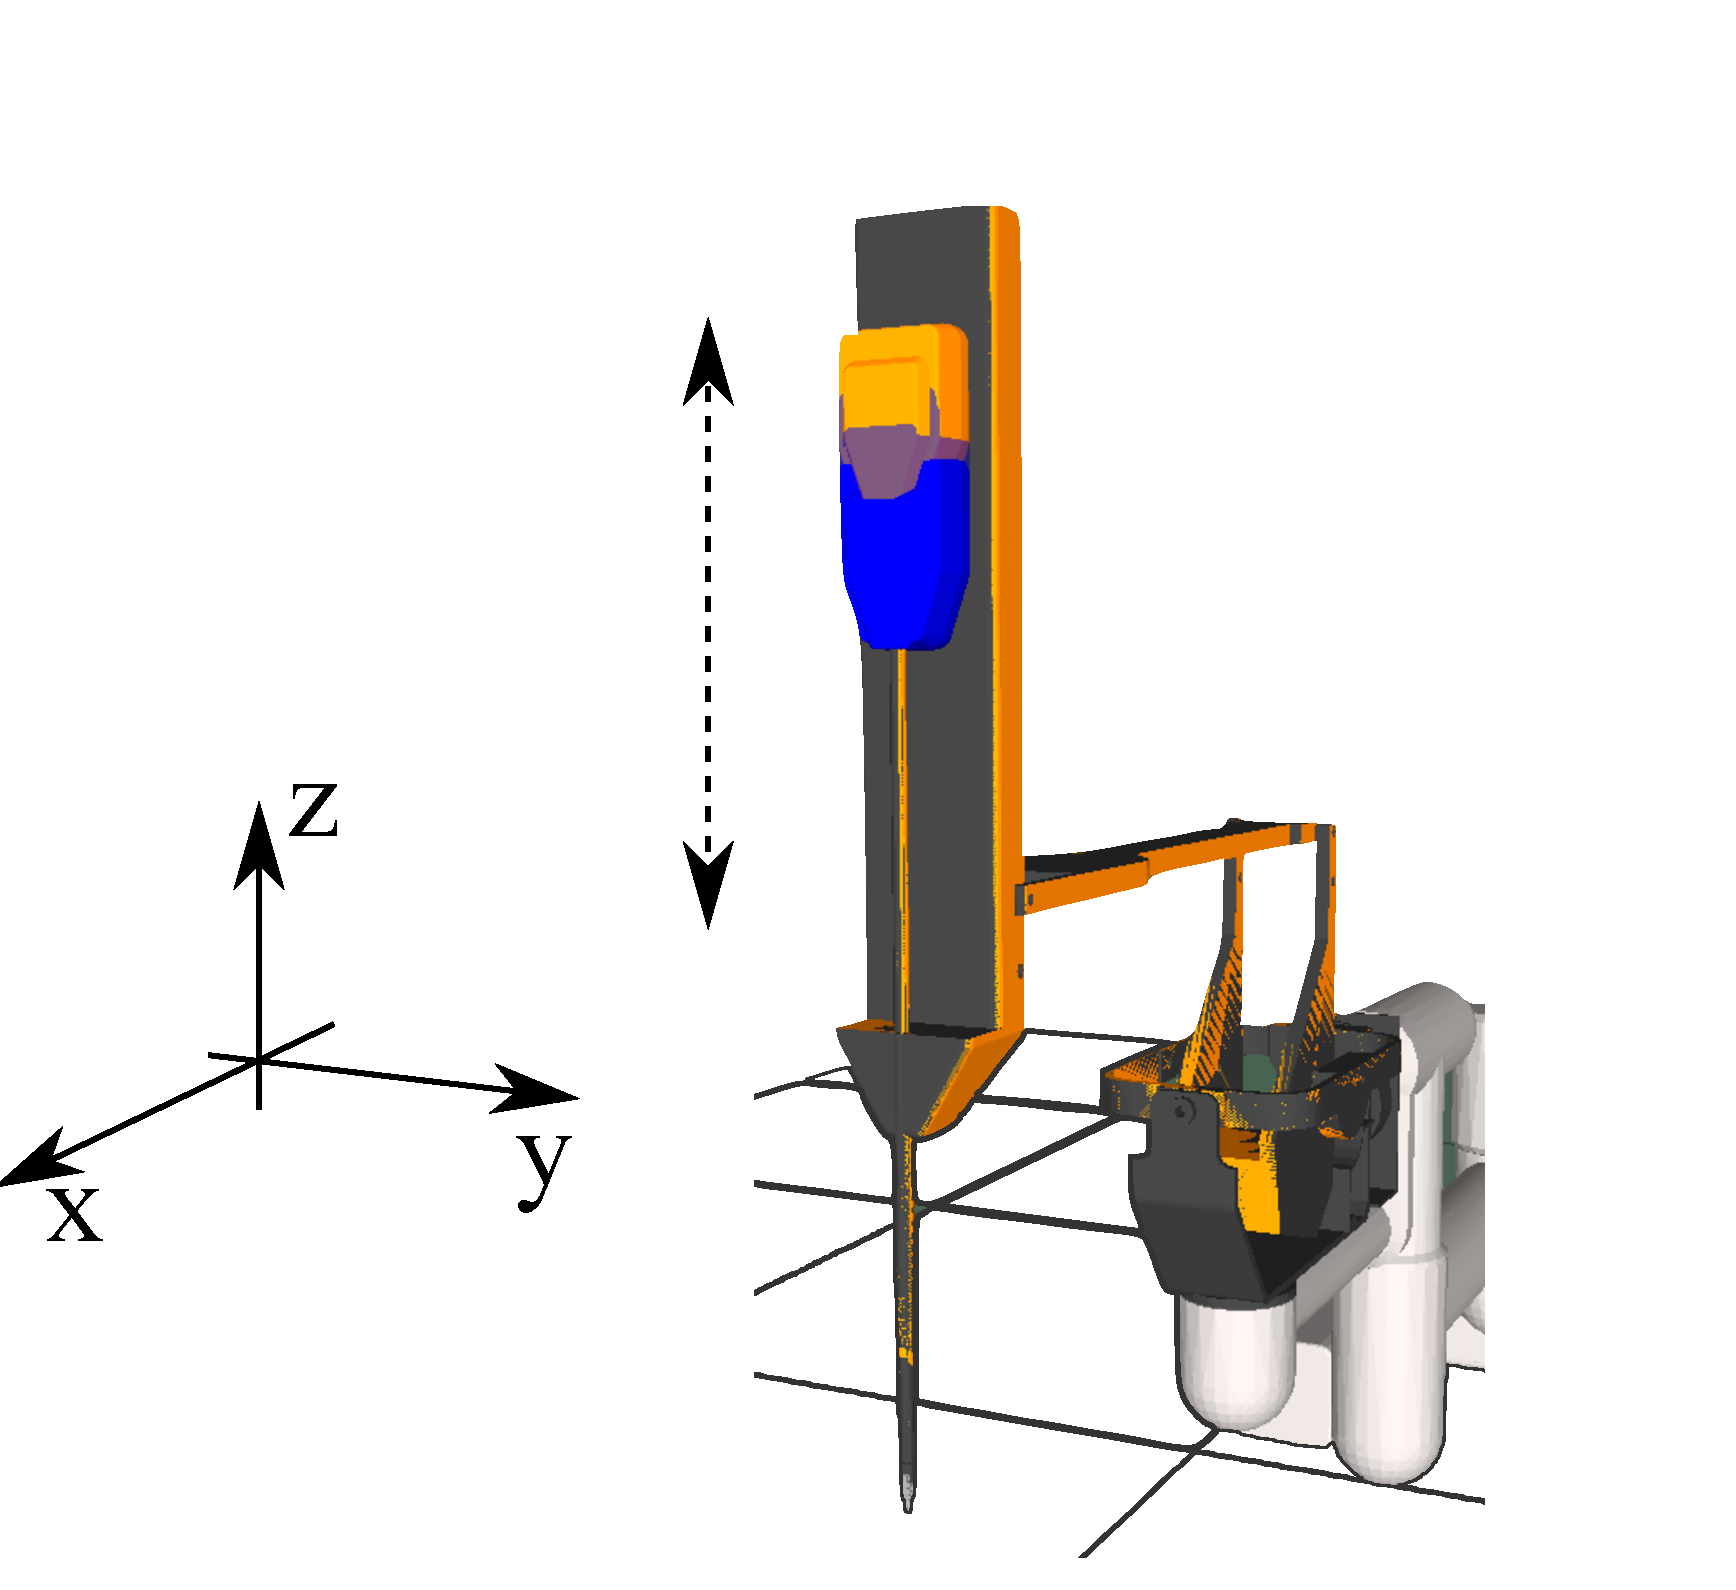
\includegraphics[width=0.46\textwidth]{slidemovefigure.pdf}\label{fig:slidefig}}%
\subbottom[Boundaries used in this chapter.]{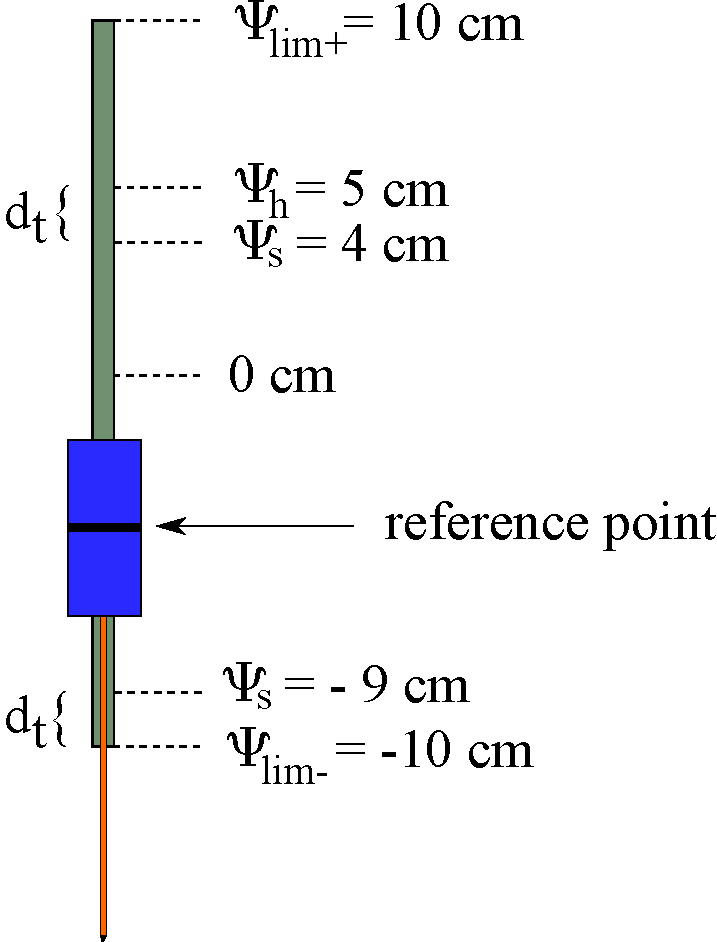
\includegraphics[width=0.42\textwidth]{slide_overview.pdf}\label{fig:safe:overview}}%
\caption{The slide position of the robotic instrument is visualized for the instrument house. As the remaining robot joints are not considered in this chapter, there is a one-to-one correspondence between instrument house position and instrument tip position. Slide house position in $x_0$ corresponds to tool tip position in zero in the $z$-dimension.}
\label{fig:slide}
\end{figure}

\vspace{-1mm}
The boundaries for the \gls{cbf} sets in slide position are summed up in \autoref{tab:intervals}.

\vspace{-1mm}
\begin{table}[H]
	\begin{tabularx}{\textwidth}{X X X }
\rowcolor{HeaderBlue} 
$\mathcal{X}$ & $\mathcal{X}_u$  & $\mathcal{X}_0$ \\
$ \mathcal{X}=\{\mathbf{x} \in[\Lambda_{\text{lim}-},\Lambda_{s-}] \cup$ \newline $\phantom{\mathcal{X}=\{\mathbf{x} \in} \,\, [\Lambda_{s+},\Lambda_{\text{lim}+}]\}$  & $\mathcal{X}_u = \{\mathbf{x} \in [\Lambda_{\text{lim}-},\Lambda_{h-}] \cup$ \newline $\phantom{\mathcal{X}_u=\{\mathbf{x} \in} \,\, [\Lambda_{h+},\Lambda_{\text{lim}+}]\} $ & $\mathcal{X}_0 = \{\mathbf{x} \in [\Lambda_{h-},\Lambda_{s-}] \cup$ \newline $\phantom{\mathcal{X}_0=\{\mathbf{x} \in} \,\, [\Lambda_{s+},\Lambda_{h+}]\}$  \\
\end{tabularx}
\caption{\gls{cbf} state intervals for the robotslide position, with limits as given in \autoref{fig:safe:overview} i.e. $\Lambda_\text{lim}$ is the physical slide limit ($\pm$0.1\,m), $\Lambda_s$ is a soft limit denoting a transition line and $\Lambda_h$ is a hard limit where a trajectory at all cost can not cross. }
\label{tab:intervals}
\end{table}
The interval $\mathcal{Y}=\{\mathbf{x} \in [\Lambda_{s-},\Lambda_{s+}]\}$ is safe thus $\tilde{u}(\mathbf{x})$ stated in \autoref{eq:utilde} can be used in this region.
As the control law stated in \autoref{eq:control_law} utilizes Lie derivatives, a system model is required before any controller design may be initiated.
%\hspace{1cm }\texttt{rostopic echo joint\_states/position[6]} \hspace{0.2cm} {\color{blue}{\# Be sure to have the ROS environment correctly configured according to \autoref{app:ros}}}

\section{Modelling of Slide Movement}\label{sec:model_slide}

\vspace{-2mm}
To obtain a model of the slide movement (along the 3D $z$-axis), the step response will be measured.  This can be done by subscribing to the \texttt{joint\_state} topic in \gls{ros} (topics are ROS syntax for communication lines, see \autoref{app:ros} for an introduction to ROS). The experiment is described in further details in \autoref{app:meas}, and the result is plotted in \autoref{fig:stepresponseslide}. 
\begin{figure}[H]
\center
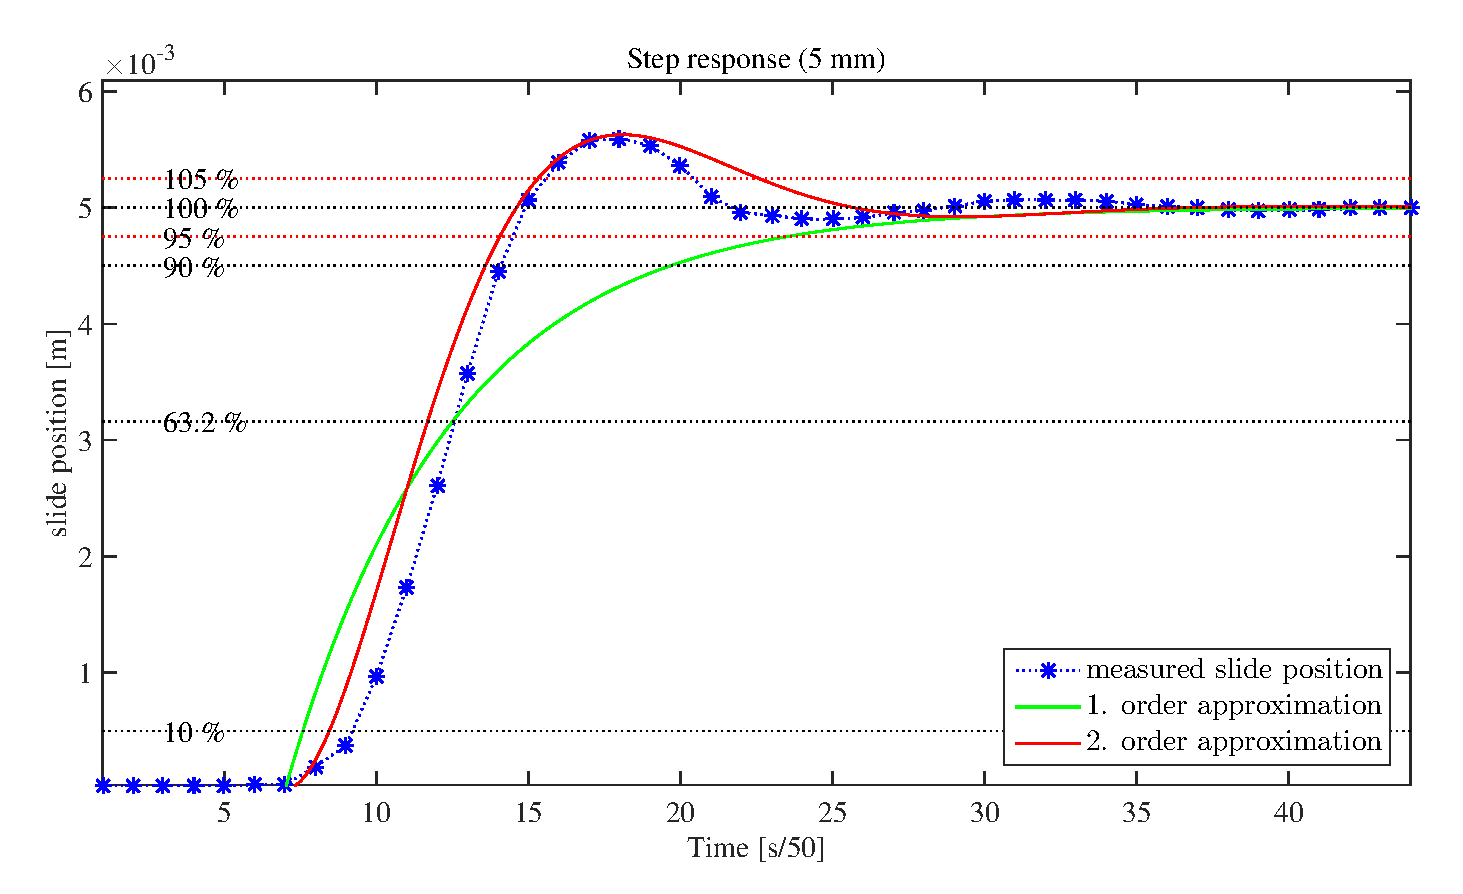
\includegraphics[scale=0.6]{step_slide.eps}
\caption{Step response from 0\,mm to 5\,mm. Plot details and measurements can be found in \autoref{app:cd} as \texttt{matlab\_scripts/slide\_step/plot\_slide\_pos.m}. The experiment is described in \autoref{app:meas}.}
\label{fig:stepresponseslide}
\end{figure}
The system can clearly be approximated with an underdamped second order model. For initial simplicity, however, a simple first order model of the slide movement is used, followed by the second order system approximation. This introduces a number of other challenges which is the reason for initial simplicity. These models of the robot slide movement  will throughout this chapter be referred to as the first and second order models, and are treated in the following way:
\vspace{-2.5mm}
\begin{itemize}
	\itemsep-0.8mm
\item The first order system model based on \textit{position} only is presented in \autoref{subsec:model_1d}. Its \gls{cbf} is constructed in \autoref{subsec:cbf-1order}, the controller designed in \autoref{sec:K_Nbar_1D_1storder}, \autoref{subsec:matlab-results-1order} shows the MATLAB implementation and finally the implementation on the da Vinci robot is presented in \autoref{subsec:implement-davinci-1d}.
\item The second order system model based on \textit{position and velocity} is presented in \autoref{subsec:model_2d}. Its \gls{cbf} is constructed in \autoref{subsec:cbf-2order}, the controller designed in \autoref{sec:K_Nbar_1D_2ndorder}, its MATLAB implementation is presented in \autoref{subsec:matlab-resutls-2-order} and finally \autoref{subsec-implement-2dmodel} documents the implementation on the da Vinci robot.
\end{itemize}
%A first order approximation of the state space system will be modelled first. 

\subsection{1D First Order Model based on Position}\label{subsec:model_1d}
\vspace{-1mm}
The system can be approximated with a linear first order system with a  time constant \gls{taus}. The time constant is read from \autoref{fig:stepresponseslide} as the time lapse from the step is applied until the state has travelled 63.2\,\% of the distance to the reference:
\vspace{-3mm}
\begin{flalign*}
\tau_s = 110\, \text{ms}
\end{flalign*} 

\vspace{-3mm}
A linear system can be outlined as:
\begin{flalign}
Y(s) &= \dfrac{1}{\tau_s s + 1}U(s) \nonumber\\
&=  \dfrac{1/\tau_s}{s + 1/\tau_s}\,U(s) = (s+1/\tau_s)^{-1}\,1/\tau_s\,U(s) \qquad\kk \overset{\overset{Y(s)=(\mathbf{C}(s\mathbf{I}-\mathbf{A})^{-1}\mathbf{B}+\mathbf{D})U(s)}{\longrightarrow}}{\scriptsize \text{compare to obtain SS form}}  \nonumber\\ 
& \dot{x} = \underbrace{-\tau_s^{-1}\,x}_{\mathbf{A}x} + \underbrace{\tau_s^{-1}}_{\mathbf{B}} u
\label{eq:1storder_1D_ss}
\end{flalign}
The system matrix \textbf{A}, input matrix \textbf{B}, output matrix \textbf{C} and feedthrough matrix \textbf{D} can be read from the above equation:
\begin{flalign}
\mathbf{A} = - \tau_s^{-1},  \kk  \kk \mathbf{B} = \tau_s^{-1}, \kk  \kk \mathbf{C} = 1 \kk \text{and} \kk \mathbf{D} = 0
\end{flalign}
This completes the first order approximation.

\subsection{1D Second Order Model based on Position and Velocity}\label{subsec:model_2d}
\vspace{-1mm}
The second order approximation has the form:
\begin{flalign}
\dfrac{Y(s)}{U(s)} = \dfrac{\omega_n^2}{s^2 + 2\zeta \omega_n s + \omega_n^2}
\label{eq:2order}
\end{flalign}
\begin{tabular}{rll} 
where  & & \\
$Y(s)$ & is the output in the Laplace domain  & [m] \\
$U(s)$ & is the input in the Laplace domain  & [m] \\
\gls{omegan} & is the natural frequency of the system & [rad/s] \\
\gls{zeta} & is the damping coefficient  & [$\cdot$] \\
\gls{s} & is the Laplace operator  & [rad/s] \\
\end{tabular}\\

The model can unambiguously be approximated from the rise time $t_r$, settling time $t_s$ (5\,\% settling time) and the overshoot $M_p$ \citep[ pp. 134-136]{bib:dynamicsystems}. They are measured  from \autoref{fig:stepresponseslide} with the purpose to find $\omega_n$ and $\zeta$:
\begin{flalign*}
\omega_n &= \dfrac{1.8}{t_r} = \dfrac{1.8}{0.106\,\text{s}} = 17 \,\text{rad/s} \\
\zeta &= \dfrac{-1}{\omega_n \cdot t_s}\log (5\,\%) = \dfrac{-1}{17 \cdot 0.320}\log(0.05) = 0.55
\end{flalign*}
\Autoref{eq:2order} can be transformed into state space form: 
\begin{subequations}
\begin{flalign*}
Y(s)s^2 + 2\zeta \omega_n Y(s) s + \omega_n^2 Y(s) - \omega_n^2 U(s)  &= 0 \\
\ddot{y}(t) + 2\zeta \omega_n \dot{y}(t) + \omega_n^2 y(t) - \omega_n^2 u(t) &= 0 
\end{flalign*}

\vspace{-4mm}
Choose $y(t) = x_1(t)$ to represent the position, and let $\dot{x}_1(t) = x_2(t)$
\begin{flalign}
\begin{bmatrix}
\dot{x}_1(t)\\\dot{x}_2(t)
\end{bmatrix} &= 
\begin{bmatrix}
0 & 1\\
-\omega_n^2  & -2\zeta \omega_n  
\end{bmatrix}
\begin{bmatrix}
x_1(t) \\ x_2(t)
\end{bmatrix} + 
\begin{bmatrix}
0\\\omega_n^2
\end{bmatrix}u(t) \label{eq:2ndorder_1D_ss}\\
y(t) &= 
\begin{bmatrix}
1 & 0
\end{bmatrix}
\begin{bmatrix}
x_1(t) \\ x_2(t)
\end{bmatrix}
\end{flalign}
\end{subequations}
\begin{tabular}{rll} 
where  & & \\
\gls{x1}$(t)$ & is the position& [m] \\
\gls{x2}$(t)$ &is the velocity  & [m/s] \\
$y(t)$ & is the output (slide position)  & [m] \\
$u(t)$ & is the control input  & [$\cdot$]\\
\end{tabular}\\

Thus the linear system matrices are:
\begin{flalign}
\mathbf{A} = \begin{bmatrix}
0 & 1\\
 -\omega_n^2   & -2\zeta \omega_n 
\end{bmatrix}, \kk  \kk \mathbf{B} = \begin{bmatrix}
0 \\ \omega_n^2
\end{bmatrix}, \kk  \kk \mathbf{C} = \begin{bmatrix}
1 & 0
\end{bmatrix} \kk \text{and} \kk \mathbf{D} = 0 \label{eq:system:2}
\end{flalign}
Which completes the second order model.

\section{Construction of CBF}\label{sec:construct_cbf}
\vspace{-2mm}
To illustrate the usefulness of \glspl{cbf}, a palpable example hereof will be created with direct application to the da Vinci robot. This example does not directly constitute application to a patient but favour the theory in a neat and comprehensible sense and secure a way to visually and physically verify the method.
%
%Consider the state intervals defined in \autoref{tab:intervals}.
%
%
\subsection{Construction of CBF Based on the First Order Model}\label{subsec:cbf-1order}
\vspace{-2mm}
In this subsection, the state vector $x \in \mathbb{R}$ consists of the position only. Thus, a parabola is now introduced as \gls{cbf} as it allows an easy way to define $\mathcal{X}_u$ and $\mathcal{X}_0$ from \autoref{tab:intervals}. %A coordinate shift is performed such that the slide movement occurs along the $x$-axis instead of the $z$-axis. 
\vspace{-2mm}
\begin{flalign}
B(x) &= ax^2+bx+c \label{eq:cbf1} 
\end{flalign}

\vspace{-4mm}
The parameters $a$, $b$ and $c$ can be easily chosen to fulfil the requirements in \autoref{cer1} and \ref{cer2} for a barrier function, thereby fulfilling the parallel requirements for the \gls{cbf} in \autoref{req1} and \ref{req3}. From \autoref{req2} it is required that either $L_gB(x) \neq 0 \,\,\,\forall x\in \mathcal{X}$, or that $L_fB(x)<0$ when $L_gB(x) = 0$, as the input in that case will not have any influence on the state. Analysing $L_gB(x) = 0$
\vspace{-1mm}
\begin{flalign*}
	L_gB(x) \Bigm|_{g(x)=\mathbf{B}} = ( 2ax + b ) \cdot \tau^{-1} = 0 \kk \Rightarrow \kk x = \dfrac{-b}{2a}\label{eq:LgB_1D}
\end{flalign*}

\vspace{-3mm}
it is seen that this is only the case in $x = \tfrac{-b}{2a}$ which is indeed the critical point for a one dimensional parabola. As is the case for Lyapunov functions (see  \autoref{eq:lyap_vdot_minus_criticalpoint}) in the critical point the requirement on the derivative is relaxed to  $L_fB(x) \leq 0$.   
\begin{flalign}
L_fB(x) = \dfrac{d}{dx}B(x)f(x)\Bigm|_{f(x)=\mathbf{A}x}  &= (2ax+b)(-\tau^{-1}x) = -2\tau^{-1}ax^2-\tau^{-1}bx \nonumber\\
L_fB(x)\Bigm|_{x= \frac{-b}{2a}} &= -2\tau^{-1}a\left(\frac{-b}{2a}\right)^2-\tau^{-1}b\left(\frac{-b}{2a}\right) = 0\nonumber
%0 \kk \Leftrightarrow \kk  -2\tau^{-1}ax^2-\tau^{-1}bx = 0 \nonumber
% \\  &-2ax^2-bx = 0 \mm \Rightarrow \mm x = 
%\begin{cases}
%  \frac{-b}{2a} \\
%   0   
%\end{cases}
\label{eq:interval1}
\end{flalign}
Hence the \gls{cbf} is valid for all choices of $a,b$. The scalar $c$ must be less than zero to comply with \autoref{req3}.
At this point in time, three equations with three unknowns can be outlined to fulfil the initial demand in \autoref{fig:safe:overview}. The value of $B(x)$ in the vertex of the parabola is within the safe region, and can thus be chosen as any \textit{negative} real number, here chosen to be -0.025.
\begin{flalign*}
 \left.
 \begin{aligned}
a\,\Lambda_{h+}^2 + b\,\Lambda_{h+} + c = 0 \\
a\,\Lambda_{h-}^2 + b\,\Lambda_{h-} + c = 0 \\
a\left( \frac{\Lambda_{h-}+\Lambda_{h+}}{2}\right)^2 + b\left(\frac{\Lambda_{h-}+\Lambda_{h+}}{2}\right) + c = -0.025
\end{aligned}
\mm \right\}
 \qquad \begin{matrix}
 a &= \,\,\,\,\,\,\,\,1.7778 \\ b &= \,\,\,\,\,\,\,\,0.0889 \\ c &= -0.0089
 \end{matrix}
\end{flalign*}
%The interval where $B(x)$ is invalid can thereby be found from \autoref{eq:interval}:
%\begin{flalign*}
%B(x) \hspace{0.15cm} \text{invalid:} \mm  x \in [-0.0250,0] \kk \text{if} \mm L_gB(x) = 0
%\end{flalign*}
%However, this is indifferent as $\{\mathcal{X} \,\bigcap\, [\Lambda_{s-},\Lambda_{s+}]  \} = \emptyset $. Thus the barrier function is a valid \gls{cbf}. It is plotted in \autoref{fig:barrierfunction}
The \gls{cbf} is plotted in \autoref{fig:barrierfunction} from which it is seen that the demands from \autoref{tab:intervals} are fulfilled.
\begin{figure}[H]
\center
	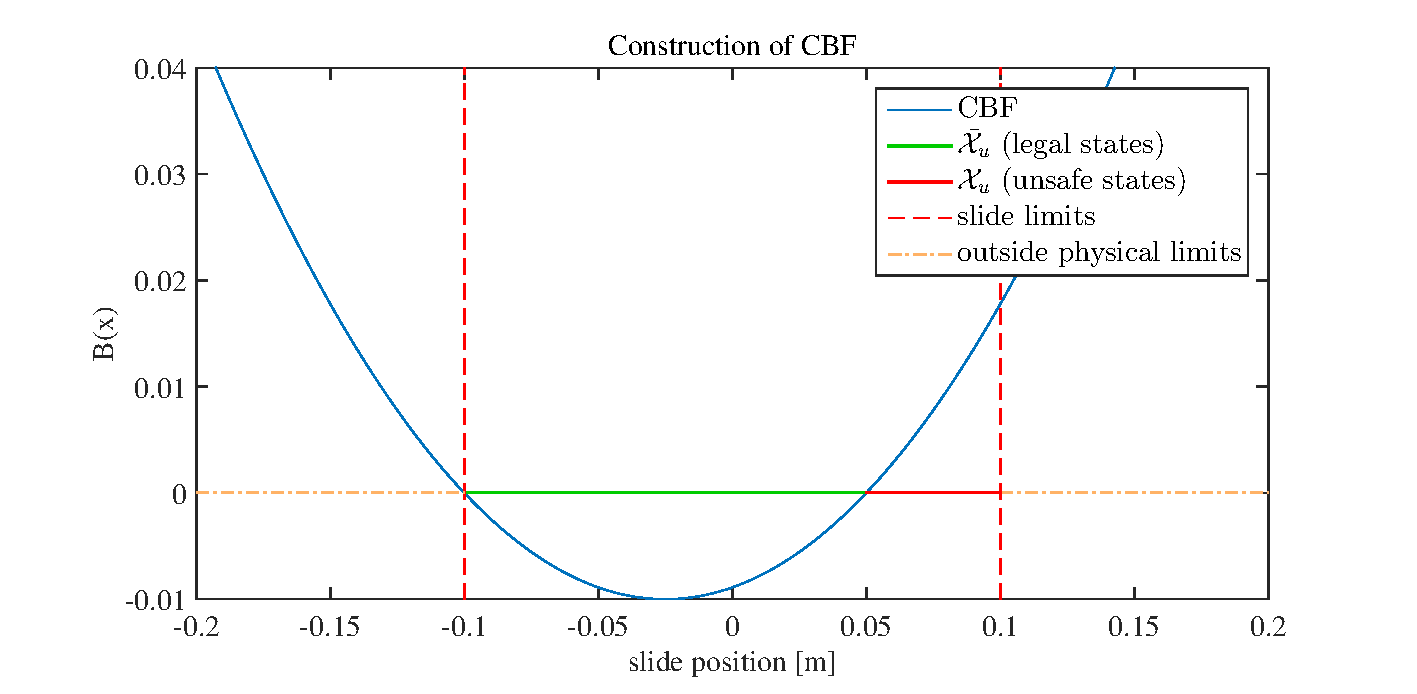
\includegraphics[scale=0.63]{parabel_1.eps}
	\caption{Barrier function shown along with the $\mathcal{X}_u$ and $\mathcal{X}_u^c$. Plot details and MATLAB script can be found in \autoref{app:cd} as \texttt{matlab\_scripts/plot\_parabola/plot\_parabola.m}}
	\label{fig:barrierfunction}
\end{figure}
%\underline{Note:} The above analysis ensures safety regardless of $L_gB(x) = 0$ as it merely takes place at the critical point, i.e.:
%\begin{flalign*}
% L_gB(x) = (2ax+b)B = 2ax\tau^{-1} + b\tau^{-1} = 0 \kk \Leftrightarrow \kk 2ax = -b \kk \Leftrightarrow \kk x = \dfrac{-b}{2a}
% \end{flalign*} 
% This is again the parabola extremity as it was found in \autoref{eq:interval1} and in fact an allowed exception for condition \autoref{req2} as the system is in its equilibrium.

\subsection{Construction of CBF Based on the Second Order model}\label{subsec:cbf-2order}
\vspace{-2mm}
Consider now for the second order system the same candidate \gls{cbf} as given in \autoref{eq:cbf1}. Note that $B(\mathbf{x})$ is a function of position only, such that the CBF is:
\vspace{-2mm}
\begin{flalign*}
B(\mathbf{x}) = a\,x_1^2+ b\,x_1 + c
\end{flalign*}

\vspace{-4mm}
For this system model the Lie derivative $L_gB(\mathbf{x})=0\,\,\forall \mathbf{x}$:
\vspace{-2mm}
\begin{flalign*}
L_gB(\mathbf{x}) = \dfrac{d B(\mathbf{x})}{d \mathbf{x}}g(\mathbf{x}) \Bigm|_{g(\mathbf{x})=\mathbf{B}} =  
\begin{bmatrix}
\dfrac{\partial B(\mathbf{x})}{\partial x_1} & \dfrac{\partial B(\mathbf{x})}{\partial x_2} 
\end{bmatrix}\begin{bmatrix}
0 \\ \omega_n^2
\end{bmatrix} = 0 \label{eq:LgB_secondorder_invalid}
\end{flalign*}
This puts forth the requirement that $L_fB(\mathbf{x})<0\,\,\, \forall \, \mathbf{x}$. Accordingly:
\vspace{-2mm}
\begin{flalign*}
L_fB(\mathbf{x}) = \dfrac{d B(\mathbf{x})}{d \mathbf{x}}f(\mathbf{x}) \Bigm|_{f(\mathbf{x})=\mathbf{Ax}} &= 
\begin{bmatrix}
\dfrac{\partial B(\mathbf{x})}{\partial x_1} & \dfrac{\partial B(\mathbf{x})}{\partial x_2} 
\end{bmatrix}
\begin{bmatrix}
0 & 1 \\
-\omega_n^2 & -2\zeta\omega_n
\end{bmatrix} \begin{bmatrix}
x_1 \\ x_2
\end{bmatrix} \nonumber \\
&= (2ax_1+b) x_2 - 0\cdot(\omega_n^2 x_1 + 2\zeta \omega_n x_2) \nonumber \\
&= (2ax_1 + b)x_2
\label{eq:2d_x1}
\end{flalign*}
As the velocity can be both decreasing and increasing for all positions, this demand is impossible to fulfil with this candidate \gls{cbf}  and it is therefore invalid. A solution is to include the velocity in the barrier function. 

Safety constraints on velocity are not of any significant importance as such, but they are necessary for $L_gB(\mathbf{x})$ to obtain values different from zero as opposed to the Lie derivative of the invalid \gls{cbf} presented above.
Consider instead the elliptic paraboloid as \gls{cbf}:
\begin{flalign}
B(\mathbf{x}) =  \left( \dfrac{(x_1-x_{10})^2}{a_2^2} + \dfrac{(x_2-x_{20})^2}{b_2^2} \right) c_1 + c_2
\label{eq:cbf2}
\end{flalign}
\begin{tabular}{rp{13.7cm}l} 
where  & & \\
$x_1$& is the position  & [m] \\
$x_2$& is the velocity & [m/s] \\
$x_{10}$& is the extremity point for $x_1$ and thereby equilibrium point for an upward paraboloid & [m] \\
$x_{20}$& is the extremity point for $x_2$ and thereby equilibrium point for an upward paraboloid & [m/s] \\
$a_2$& is a constant that dictates the level of curvature in the $x_1-B(\textbf{x})$ plane & [$\cdot$] \\
$b_2$& is a constant that dictates the level of curvature in the $x_2-B(\textbf{x})$ plane & [$\cdot$] \\
$c_1$ & is a constant that dictates if the paraboloid points upward ($c_1>0$) or downward ($c_1 < 0$)& [$\cdot$]  \\
$c_2$ & is a constant that dictates the offset in $B(\textbf{x})$ axis & [$\cdot$] \\
\end{tabular}\\

The elliptic paraboloid allows constraints on both position and velocity.  To ensure that the position demands from \autoref{tab:intervals} are still fulfilled and are so for all possible velocities (constrained by the slide movement's physical limits), the below values are chosen:
\begin{flalign*}
x_{10} &= \dfrac{\Lambda_{h-}+\Lambda_{h+}}{2} = -0.025 \\
x_{20} &= 0\\
M_{0} &= 4
%\Lambda_{x2-} &= -4 \kk \text{denotion of the lowest value where $B(0,x_2)=0$} \\
%\Lambda_{x2+} &= 4 \kk \text{denotion of the highest value where $B(0,x_2)=0$} 
\end{flalign*}
where \gls{M0} denotes the semimajor axis of the zero level set of the \gls{cbf}.
Note that $x_{20}$ ensures velocity equilibrium in 0\,m/s and note that the velocity outermost points are determined far bigger than the robot's physical limits to ensure that all position values on the interval  $[-0.1\,\,\,\,0.05]$ are considered safe (almost) independently of the velocity. % $\mathcal{X}_0 \notin \mathcal{X}_u $. 
This is sketched in \autoref{fig:cbf_2ndorder} along with the chosen values.
\begin{figure}[htbp]
	\centering
	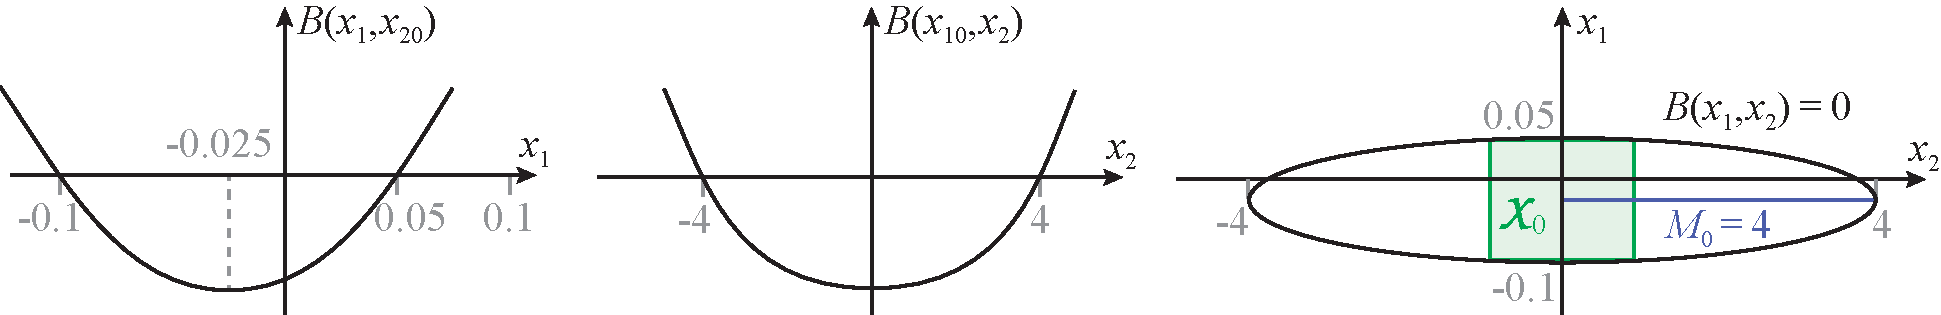
\includegraphics[width=\textwidth]{cbf_2ndorder.pdf}
	\caption{Choice of critical point coordinate $x_{10}$  as the middle of the safe position interval. The semimajor axis of the \gls{cbf}'s zero level set is chosen much larger than the physical limits  of the slide velocity.}
	\label{fig:cbf_2ndorder}
\end{figure}

Having chosen the coordinates $x_{10}$ and $x_{20}$ for the critical point, an arbitrary negative value is chosen for $B(x_{10},x_{20})$. Using the four known coordinates from the zero level set $(\Lambda_{h+},x_{20})$, $(\Lambda_{h-},x_{20})$, $(x_{10},-M_0)$ and $(x_{10},M_0)$, five equations with four unknowns can be outlined with the below numerical values.

\vspace{-3mm}
\begin{flalign*}
\hspace{5mm} \left.
\begin{aligned}
\left( \dfrac{\left(\frac{\Lambda_{h-}+\Lambda_{h+}}{2}-x_{10}\right)^2}{a_2^2} + \frac{(0-x_{20})^2}{b_2^2} \right)c_1 + c_2 =  {-1.000} \\
\left(\dfrac{(\Lambda_{h+}-x_{10})^2}{a_2^2} +\frac{(0-x_{20})^2}{b_2^2}\right) c_1 + c_2 = 0 \\
 \left(\dfrac{(\Lambda_{h-}-x_{10})^2}{a_2^2}+\frac{(0-x_{20})^2}{b_2^2}\right) c_1 + c_2 = 0 \\
 \left(\dfrac{\left(\frac{\Lambda_{h-}+\Lambda_{h+}}{2}-x_{10}\right)^2}{a_2^2} +\dfrac{(4-x_{20})^2}{b_2^2} \right)c_1 + c_2 = 0 \\
\left(\dfrac{\left(\frac{\Lambda_{h-}+\Lambda_{h+}}{2}-x_{10}\right)^2}{a_2^2} + \dfrac{(-4-x_{20})^2}{b_2^2}\right) c_1 + c_2 = 0 
% \dfrac{\left(0-x_{20}\right)^2}{b_2^2} c_1 + c_2 =  \underbrace{-1.000}_\text{any constant $<0$}  
\end{aligned}
\mm \right\}
 \qquad 
\begin{matrix*}[r]
x_{10} &=& -0.025 \\ 
x_{20} &=&  0.000 \\
B(x_{10},x_{20}) &=&   -1.000\\
&&\\
a_2 &=& 0.075 \\ 
b_2 &=& 4.000 \\
c_1 &=& 1.000 \\ 
c_2 &=& -1.000
\end{matrix*}
\end{flalign*}
The Lie derivatives can now be calculated as:
\begin{flalign}
L_gB(\mathbf{x}) &= \dfrac{d B(\mathbf{x})}{d \mathbf{x}}  g(\mathbf{x}) \Big|_{g(\mathbf{x})=\textbf{B}} = \begin{bmatrix}
\dfrac{\partial B(\mathbf{x})}{\partial x_1} & \dfrac{\partial B(\mathbf{x})}{\partial x_2}
\end{bmatrix}  \begin{bmatrix}
0 \\ \omega_n^2
\end{bmatrix} \nonumber \\
 &= \begin{bmatrix}
 \dfrac{c_1(2x_1 - 2x_{10})}{a_2^2} &  \dfrac{c_1(2x_2 - 2x_{20})}{b_2^2}
\end{bmatrix}  \begin{bmatrix}
0 \\ \omega_n^2
\end{bmatrix} = 
\dfrac{c_1\omega_n^2(2x_2-2x_{20})}{b_2^2} \Bigm|_{x_{20}=0} \nonumber\\
&= \dfrac{2c_1\omega_n^2}{b_2^2} x_2
\label{eq:LgB_2}
\end{flalign}
It is seen that $L_gB(\mathbf{x}) \neq 0 \mm \forall \,\,\, x_2 \neq 0$, hence $L_fB(\mathbf{x})$ is for that reason analysed and evaluated at $x_2=0$:
%\vspace{-3mm}
\begin{flalign}
L_fB(\mathbf{x}) &= 
\dfrac{\partial B(\mathbf{x})}{\partial \mathbf{x}} f(\mathbf{x})
\Big|_{f(\mathbf{x}) = \textbf{\textbf{Ax}}} =
\begin{bmatrix}
\dfrac{\partial B(\mathbf{x})}{\partial x_1} & \dfrac{\partial B(\mathbf{x})}{\partial x_2}
\end{bmatrix} 
\begin{bmatrix}
0 & 1 \\
-\omega_n^2 & -2 \zeta \omega_n
\end{bmatrix} 
\begin{bmatrix}
x_1 \\ x_2
\end{bmatrix} \nonumber\\
&= \begin{bmatrix}
 \dfrac{c_1(2x_1 - 2x_{10})}{a^2} &  \dfrac{c_1(2x_2 - 2x_{20})}{b^2}
\end{bmatrix} 
\begin{bmatrix}
x_2 \\ -\omega_n^2 x_1 - 2\zeta \omega_n x_2
\end{bmatrix} \nonumber\\
&= \dfrac{c_1x_2(2x_1-2x_{10})}{a_2^2} - \dfrac{c_1(2x_2-2x_{20})(\omega_n^2 x_1+2\zeta \omega_n x_2 )}{b_2^2} \Big|_{x_{20} = 0} \nonumber\\
&= 2c_1\left( \dfrac{x_1-x_{10}}{a_2^2} - \dfrac{\omega_n^2 x_1 +2\zeta \omega_n x_2}{b_2^2} \right) x_2 \Big|_{x_{2} = 0} = 0
\label{eq:LfB_2}
\end{flalign}

It is noted that $L_fB(\mathbf{x}) = 0$ for all points $(x_1,0)$ (i.e. at zero velocity) which % implies stability but not asymptotic stability. That is in general not good for physical systems and 
does not fulfil \autoref{req2}. It does, however, fulfil \autoref{req2_weak} thus proving $B(\mathbf{x})$ from \autoref{eq:cbf2} to be a weak \gls{cbf}. %However, an engineering reflection and decision is taken at this point.
Note that when the velocity is zero, the slide movement is stable, although only marginally stable. %At this point $k_0(x)=0$, which indeed will force the slide movement to its origin as the control signal is the reference to a position controller. 
As an engineering reflection it is considered that when the state leaves the marginally stable equilibrium, $x_2 \neq 0$,  the safety controller  will ensure that the state will increase its distance to the unsafe set and move towards its stable equilibrium in $(x_{10},x_{20})=(-0.025,0)$. 
%It implies hereafter $x_2 \neq 0$ again which is sufficient for the safety controller. %That is in this case a good thing as the slide will move back to the safe region and away from $\Lambda_{h-}$ and $\Lambda_{h+}$. Lastly, the velocity will never be truly zero due to the finite resolution, i.e. a finite sampling rate. For these reasons, the \gls{cbf} from \autoref{eq:cbf2} is accepted, well aware that the \gls{cbf} is insufficient,. It is, however, important to keep in mind that this is a dangerous decision. {\color{green}{RAFAL: Er det overhovedet OK at sige s\aa dan?}}


\begin{figure}[H]
\hspace*{-5mm}
	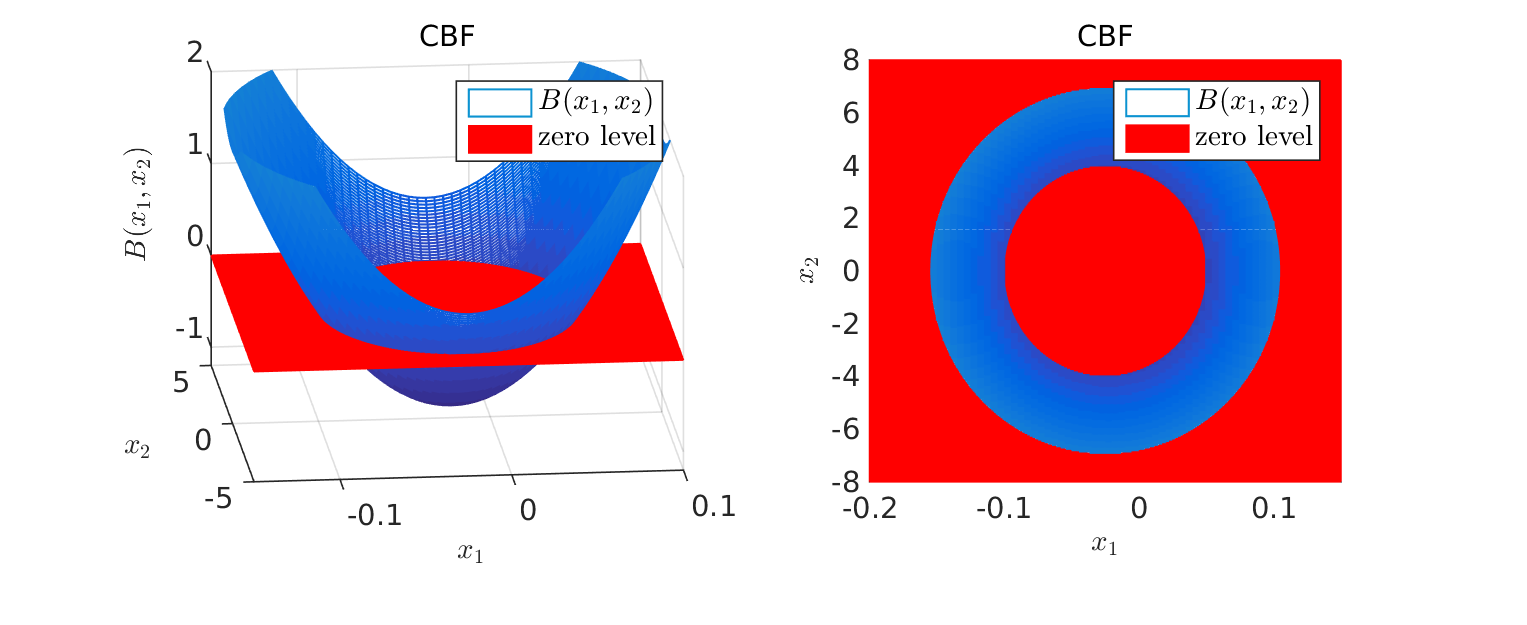
\includegraphics[width=1.1\textwidth]{cbf_2d.eps}
	\vspace*{-11mm}
	\caption{CBF for the second order system model. In the right plot the curve is seen from "above" for comparison with \autoref{fig:cbf_2ndorder}. Plot details and MATLAB script can be found in \autoref{app:cd} on the path \texttt{matlab\_scripts/plot\_cbf\_2d/plot\_cbf\_2d.m}}
	\label{fig:barrierfunction_2d}
\end{figure}
The elliptic paraboloid with its proper boundaries is plotted in \autoref{fig:barrierfunction_2d}, from which it is seen how $B(\mathbf{x})<0$ only within the specified region, and positive for all $\mathbf{x}\in [\Lambda_{h-},\Lambda_{h+}]\times[-M_0,M_0] $. %, and thus everything else is unsafe, i.e. $B(x) > 0$. 
It is also seen that for small velocities (physically $x_{2,\text{max}}\approx 0.5$\,m/s) the \gls{cbf} forms a nearly square subset of the safe set, i.e. $\{\mathbf{x}\in[-0.1,0.05]\times[-0.5,0.5] \}$, %is approximately vertical in the boundaries of $x_1$ %when the big numerical difference in the axes is taken into account.
leaving $\mathcal{X}_0$ almost independent of the velocity in this area, as prescribed in \autoref{fig:cbf_2ndorder}.

\vspace{5mm}
\begin{figure}[H]
	\centering
	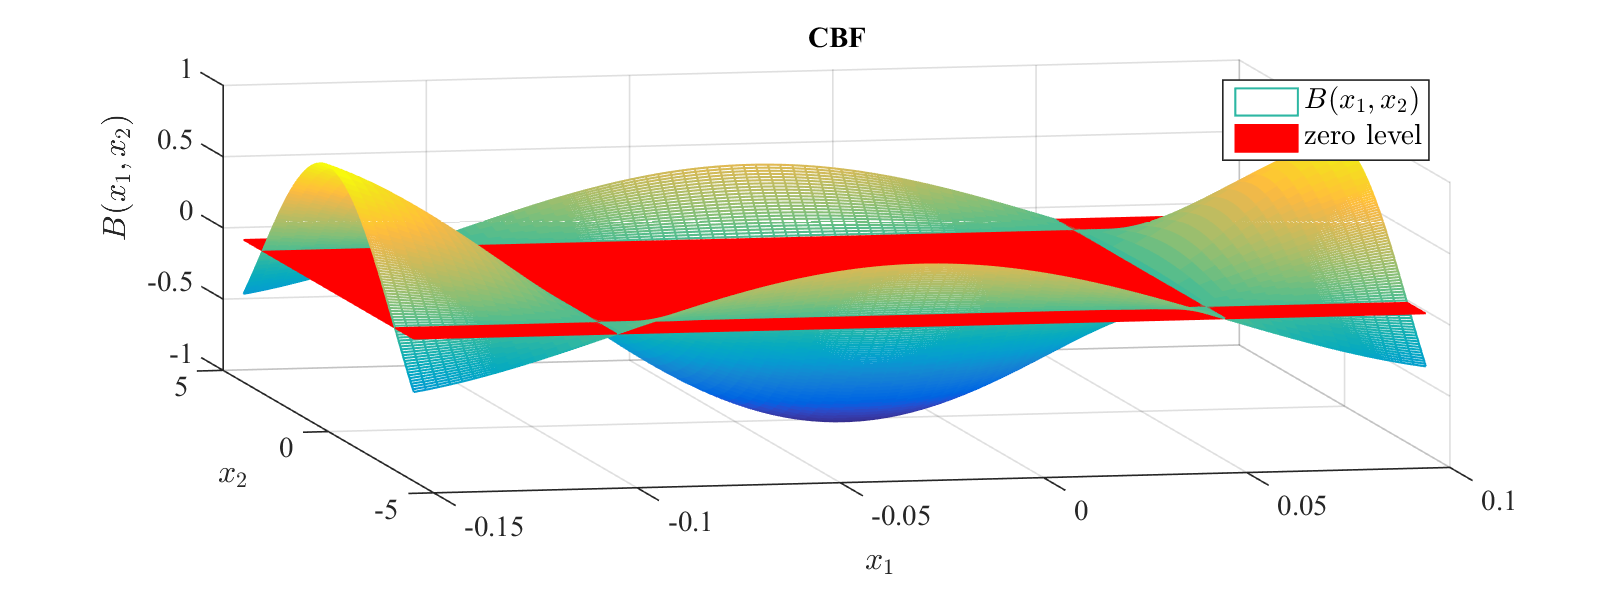
\includegraphics[width=\textwidth]{cbf_example_sinus.eps}
	\caption{CBF. Example to demonstrate how other CBFs suffer when $x_2 = 0$.}
	\vspace{-7mm}
	\label{fig:barrierfunction_example_sinus}
\end{figure}
\vspace{8mm}

\textbf{\underline{\textit{Remark:}}} The issue caused by $x_2=0$ is not only the case for this specific \gls{cbf} but for many \gls{cbf}s. Take for example another CBF that could fulfil the position requirements from \autoref{tab:intervals}:
\begin{flalign*}
B(\mathbf{x}) = \cos (c_3 x_1 + c_4) \cdot \cos (c_5 x_2 + c_6)
\end{flalign*}
It turns out that the coefficients $c_3 = 21.00, c_4 = 119.91, c_5 = 0.50, c_6 = 3.15$ induce a CBF with the same properties as the one depicted in \autoref{fig:barrierfunction_2d}. The \gls{cbf} is outlined graphically in \autoref{fig:barrierfunction_example_sinus}.


Thus $L_gB(\mathbf{x})$ can be found as:
\vspace{-3mm}
\begin{flalign*}
L_gB(\mathbf{x}) = -c_5 \omega_n^2 \cos (c_3 x_1+c_4)\sin(c_5 x_2+c_6)
\end{flalign*}

\vspace{-3mm}
Now note that $L_gB(\mathbf{x}) = 0$ when $c_6+c_5x_2 = i\pi$, $i\in\mathbb{Z}$, which is true for e.g. $x_2 \approx 0$. This implies the requirement that $L_fB(\mathbf{x}) < 0$ whenever $x_2 \approx 0$. % As $L_gB(x_1,x_2) \neq 0 \,\, \forall \,\, x_2 \approx 0$, requirements for $L_fB(x_1,x_2)$ is necessary. 
However, taking a look at $L_fB(\mathbf{x})$:
\begin{flalign*}
L_fB(\mathbf{x}) = 
c_5\cos (c_3 x_1+c_4 ) \sin(c_5 x_2+c_6)( \omega_n^2 x_1 + 2  \zeta \omega_n x_2) - c3 x_2 \cos( c_5 x_2+c_6) \sin( c_3 x_1+c_4)
\end{flalign*}
quickly poses the fact that $L_fB(\mathbf{x})$ is not necessarily negative for $x_2 \approx 0$ due to the sign alternation caused by the term $\sin(c_3 x_1+c_4)$ in the boundaries.

\section{Control Design}
\vspace*{-1mm}
This section constitutes the design of the two controllers. The controller based on the first order approximation is straight forward whereas the controller based on the second order approximation requires an observer because  velocity  measurements are not available through ROS in the current setup.

\subsection{Control Design Based on the First Order Model}\label{sec:K_Nbar_1D_1storder}
\vspace*{-1mm}
To be able to find $k_0(x)$ from \autoref{eq:control_for_safety}, the constant $\epsilon$ used in \autoref{eq:smoothness} must be found. It can be determined from the \gls{cbf} from \autoref{eq:cbf1} such that it complies with the requirements from \autoref{tab:intervals}:
\begin{flalign}
\epsilon = |B(\Lambda_{s+})| = |B(\Lambda_{s-})| = 0.00249
\label{eq:epsilon}
\end{flalign}
Utilizing $\sigma(x)$ as described in \autoref{eq:smoothness} secures a neat way to incorporate the transition between the position controller and the safety controller $k_0(x)$, the latter which which gradually takes over when the trajectory exceeds $\Lambda_s$  and has fully taken over when the trajectory reaches $\Lambda_h$. \Autoref{fig:epsilon_plot} illustrates how $\epsilon$ and $B(x)$ are connected.
\begin{figure}[H]
	\center
		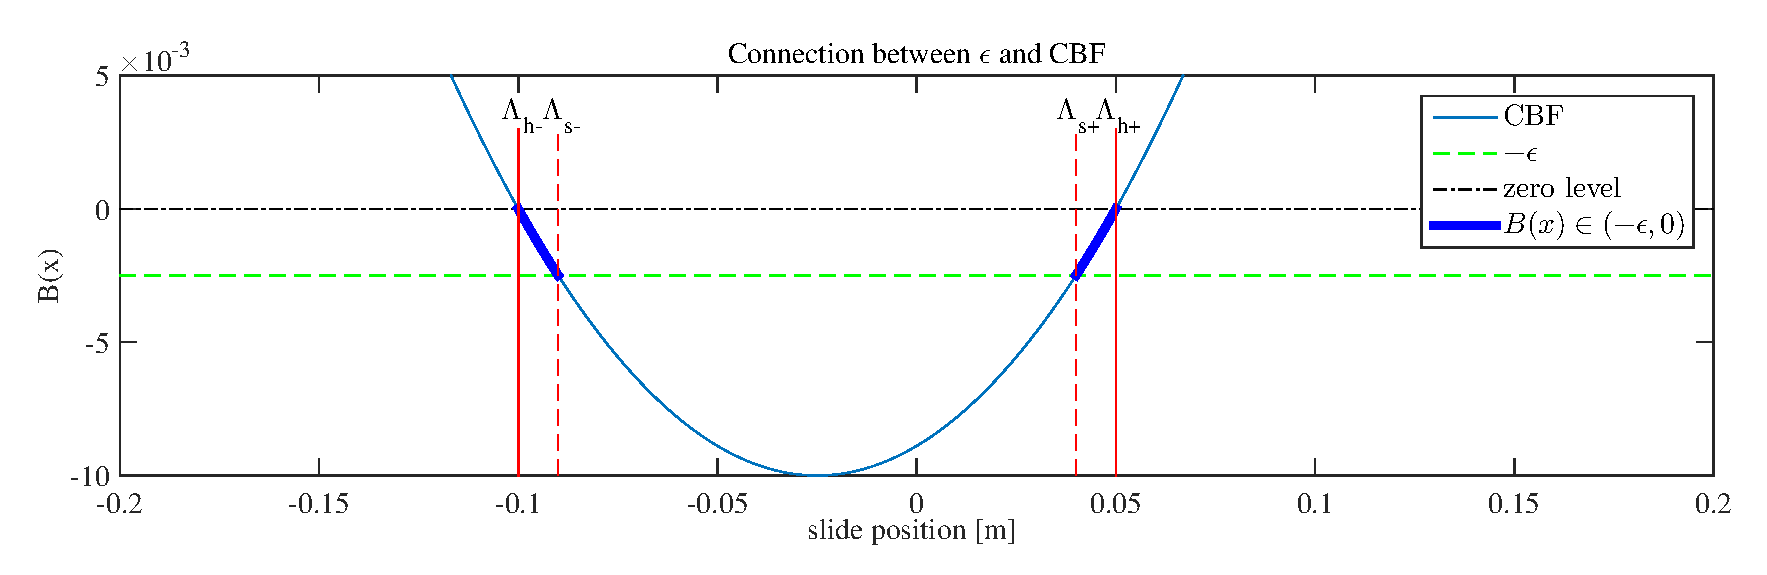
\includegraphics[scale=0.55]{epsilon_plot.eps}
	\caption{Connection between $\epsilon$ and CBF. MATLAB script and plot details can be found in \autoref{app:cd} as \texttt{matlab\_scripts/plot\_epsilon/plot\_epsilon\_slide\_1d.m}}
	\label{fig:epsilon_plot}
\end{figure}

The system is approximated as a linear system on the form $\dot{\mathbf{x}}=\textbf{Ax}+\textbf{Bu}$, thus pole placement can be used. No constraints to the constant feedback matrix $\mathbf{K}$ will be outlined except stability. It will therefore be determined from the pole placement method where a closed loop pole that is ten times faster than the open loop pole will be placed. Ackermann's formula can be used \citep{bib:acker}:
\begin{enumerate}
\itemsep-3mm
\item Identify the desired closed loop polynomial as $\textbf{A}_{cl}(s) = s^n + a_{c(n-1)}s^{n-1}  +  \cdots + a_ {c1}s + a_{c0}$: 
\vspace*{-1mm}
\begin{flalign*}
\textbf{A}_{cl}(s) = s + 10\,\tau^{-1}
\end{flalign*}
\item Identify the open loop polynomial as $\textbf{A}_{ol}(s) = s^n + a_{n-1}s^{n-1} +  \cdots + a_1s + a_0$: 
\vspace*{-1mm}
\begin{flalign*}
\textbf{A}_{ol}(s) = \lambda + \tau^{-1}
\end{flalign*}
\item Compute the feedback matrix in controllable canonical form:
\vspace*{-1mm}
\begin{flalign*}
 \bar{\mathbf{K}}^T = \begin{bmatrix}   
 \bar{k_1} \\
 \vdots \\
 \bar{k_n}
 \end{bmatrix} = \begin{bmatrix}
 a_{c0} - a_0 \\
 \vdots \\
 a_{c(n-1)} - a_{n-1}
 \end{bmatrix} \kk \Rightarrow  \kk \bar{\mathbf{K}}^T = 10\,\tau^{-1} - \tau^{-1} = 9\,\tau^{-1}
\end{flalign*}
\vspace*{-1mm}
\item Compute the similarity transform $Q$ recursively as: 
\vspace*{-1mm}
\begin{flalign*}
\textbf{Q} = \begin{bmatrix}
\textbf{q}_1 & \textbf{q}_2 & \cdots & \textbf{q}_n
\end{bmatrix} \qquad
\Rightarrow \qquad
\textbf{Q} = \tau^{-1}
\end{flalign*}
\vspace*{-1mm}
\begin{tabular}{rl}
where&\\
$ \textbf{q}_n$&\hspace{-3mm}$ = \textbf{B}$ \\
$ \textbf{q}_{j-1}$&\hspace{-3mm}$ = \textbf{A}\,\textbf{q}_j + a_{j-1}\textbf{B}$\\
\end{tabular}\\\\

\item Compute the feedback matrix as:
\vspace*{-1mm}
\begin{flalign}
\mathbf{K} = \bar{\mathbf{K}}\,\mathbf{Q}^{-1} = 9\,\tau^{-1}\dfrac{1}{\tau^{-1}} = 9
\label{eq:K_1}
\end{flalign}
\end{enumerate}
The constant feedback matrix $\bar{\mathbf{N}}$, ensuring unity gain between reference and output, can be computed as \citep{bib:Nbar}:
\vspace*{-3mm}
\begin{flalign}
\bar{\mathbf{N}} = - \left( \mathbf{C}\,\mathbf{A}_{cl}^{-1}\,\mathbf{B} \right)^{-1} =  - \left( \mathbf{C}\,(\mathbf{A}-\mathbf{B}\,\mathbf{K})^{-1}\,\mathbf{B} \right)^{-1} = 10
\label{eq:barm_1}
\end{flalign}
%\subsubsection*{Merged Control Law}
With the Lie derivatives computed as:
\begin{flalign}
L_fB(\mathbf{x}) = -2a\tau^{-1}x^2-b\tau^{-1}x \kk \wedge \kk L_gB(\mathbf{x}) = 2a\tau^{-1}x + b\tau^{-1}
\label{eq:lies_1}
\end{flalign}


\begin{recap}[Control Law for First Order Approximation]\label{recap:1d_static_1storder}

	The complete control law can be determined from \autoref{eq:control_law}:
\begin{flalign*}
u(x) = \sigma(x)k_0(x)+(1-\sigma(x))(\bar{\mathbf{N}}  x_\text{ref}-\mathbf{K}x) 
\end{flalign*}
\vspace{-0.8cm}
\begin{tabular}{rp{13.7cm}} 
where  & \\
$\sigma(x)$ & is computed from \autoref{eq:smoothness} with the $\epsilon$ found in \autoref{eq:epsilon} and the \gls{cbf} found in \autoref{eq:cbf1}  \\
$k_0(x)$ & is computed from \autoref{eq:control_law_safety} with the Lie derivatives stated in \autoref{eq:lies_1} \\
$\bar{\mathbf{N}}$ & is found in \autoref{eq:barm_1}  \\
$\mathbf{K}$ & is found in \autoref{eq:K_1} \\
\end{tabular}\\
\end{recap}
%\vspace{-0.2cm}
This completes the control design based on a first order system approximation. 



\subsection{Control Design Based on the Second Order Model}\label{sec:K_Nbar_1D_2ndorder}
\vspace{-2mm}
A necessary condition for a controller is that the system is controllable:
\vspace{-1mm}
\begin{flalign*}
 \mathbf{\mathcal{C}} = \begin{bmatrix}
 \mathbf{B} & \mathbf{A}\,\mathbf{B}
 \end{bmatrix} =  \begin{bmatrix}
 0 & \omega_n^2 \\
 \omega_n^2 & -2 \zeta \omega_n^3
 \end{bmatrix} \kk \text{thus} \mm \text{rank} ( \mathcal{C} ) = 2 = n \kk \Rightarrow \mm \text{controllable}
\end{flalign*} 

\vspace{-3mm}
To design the smoothing in the transition space $\mathcal{T}$ for the second order approximation, $\epsilon$ is found as the level set value of $B(\mathbf{x})$ at the position soft limit with zero velocity:
\vspace{-1mm}
\begin{flalign}
	\epsilon = |B(\Lambda_{s+},x_{20})| = |B(\Lambda_{s-},x_{20})| = 0.2489
	\label{eq:epsilon_2}
\end{flalign}

%\autoref{eq:epsilon} is used again such that the \gls{cbf} from \autoref{eq:cbf1} is reused here. To allow the instrument some physical distance to brake and turn around (caused by the inertia), $\sigma(\mathbf{x})$ is multiplied by a scalar $c$ such that it reaches 1 before it is too late for the instrument to turn around. $\sigma(\mathbf{x})$ is however still limited to its maximum value at 1.
%\begin{flalign}
%\sigma(\mathbf{x}) = 
%\begin{cases}
%0 & \text{if} \mm B(x_1) \leq -\epsilon \\
%c\, \left( -2  \left( \dfrac{B(x_1)}{\epsilon} \right)^3 - 3\left( \dfrac{B(x_1)}{\epsilon} \right)^2 +1 \right) \kk &\text{if} \mm B(x_1) \in (-\epsilon,0) \\
%1  &\text{if} \mm B(x_1) \geq 0
%\end{cases}
%\end{flalign} 
\vspace{-3mm}
At this point, two cases will be considered:
\vspace{-3mm}
\begin{itemize}
	\itemsep-1mm
\item \textbf{1.} Construction of $\mathbf{K}$ and $\bar{\mathbf{N}}$ in a similar way as in \autoref{sec:K_Nbar_1D_1storder}. This is possible in an ideal simulation because the velocity can be extrapolated by means of the forward Euler approach (ideal design).
\item \textbf{2.} Development of an observer to estimate the velocity based on the model and position measurements. This is necessary on a real system.
\end{itemize}

\vspace{-3mm}
\subsubsection{Controller Design for MATLAB Simulation}
\vspace{-2mm}
The design of $\mathbf{K}$ and $\bar{\mathbf{N}}$ will follow the exact same procedure as described for the first order model except now $\mathbf{K} \in \mathbb{R}^{1 \times 2}$, while $\bar{\mathbf{N}}$ remains as a scalar. The entire design procedure is therefore not elaborated.  

However, it is of interest to slow down the system dynamics slightly compared to the controller based on a first order system. This is to enter the transition region with a lower velocity and thereby allow the safety controller some transition space to navigate the trajectory back to its safe area. The eigenvalues of the second order system is found to:
\vspace{-4mm}
\begin{flalign*}
\lambda_\text{2nd order system} = \begin{cases}
-10.295 -14.765\,j \\
-10.295 +14.765\, j
\end{cases}
\end{flalign*}

\vspace{-3mm}
The feedback vector can be found with the MATLAB command \texttt{acker} based on pole placement slightly faster than the system itself.
\vspace{-2mm}
\begin{flalign}
\mathbf{K} = \texttt{acker(A,B,C,D,[-40 -50])} = \begin{bmatrix}
5.173  &  0.214
\end{bmatrix}
\label{eq:K_2}
\end{flalign}

\vspace{-3mm}
The DC gain can now be corrected with:
\vspace{-1mm}
\begin{flalign}
\bar{\mathbf{N}} = - \left( \mathbf{C}\,\mathbf{A}_{cl}^{-1}\,\mathbf{B} \right)^{-1} =  - \left( \mathbf{C}\,(\mathbf{A}-\mathbf{B}\,\mathbf{K})^{-1}\,\mathbf{B} \right)^{-1} = 6.173
\label{eq:Nbar_2}
\end{flalign}

\vspace{-3mm}
These matrices are used in the MATLAB simulation.

\subsubsection{Observer Design for Implementation on the da Vinci Robot}
\vspace{-2mm}
As the \gls{cbf} and hence the safety controller are functions of both position and velocity of the end effector, measurements of both are needed. For the present setup, however, velocity measurements are not available through ROS, and thus an observer is designed to estimate the velocity.
A necessary condition for an observer is that the system is observable:
\begin{flalign*}
 \mathbf{\mathcal{O}}= \begin{bmatrix}
 \mathbf{C} \\ \textbf{CA}
 \end{bmatrix} =  \begin{bmatrix}
 1 & 0 \\
 0 & 1
 \end{bmatrix} \kk \text{thus} \mm \text{rank} ( \mathcal{O}) = 2 = n \kk \Rightarrow \mm \text{observable}
\end{flalign*} 
An observer (discrete version) with proper gain corrections can be designed as \citep{bib:Nbar}:
\begin{flalign}
\hat{\mathbf{x}}(k+1) = \boldsymbol{\Gamma} \hat{\mathbf{x}}(k) + \boldsymbol{\Phi} \mathbf{K}_d \hat{\mathbf{x}}(k) + \mathbf{L}_d ( \underbrace{\mathbf{C}\hat{\mathbf{x}}(k)-\mathbf{y}(k)}_\text{error} ) + \mathbf{M} x_\text{ref}
\label{eq:observer}
\end{flalign}

\vspace{-4mm}
with the associated continuous system:
\vspace{-1mm}
\begin{flalign*}
	\dot{\mathbf{x}} &= \textbf{Ax} + \mathbf{B}(\mathbf{N} x_\text{ref} - \textbf{Kx}) \\
	\textbf{y} &= \textbf{Cx}
\end{flalign*}
\begin{tabular}{rl} 
where  & \\
$k$& is the current sample \\
\gls{Gamma}& is the discretized system matrix \\
\gls{Phi}& is the discretized input matrix \\
\gls{Kd}& is control gain calculated from the discretized matrices \\
\gls{Ld}& is observer gain calculated from the discretized matrices \\
\gls{M}& is gain correction to ensure unity gain for the observer \\
\gls{N}& is gain correction to ensure unity gain for the system \\ 
\end{tabular}\\


The equations are implemented in simulink as shown in \autoref{fig:simulink_observer}.
\begin{figure}[H]
	\center
		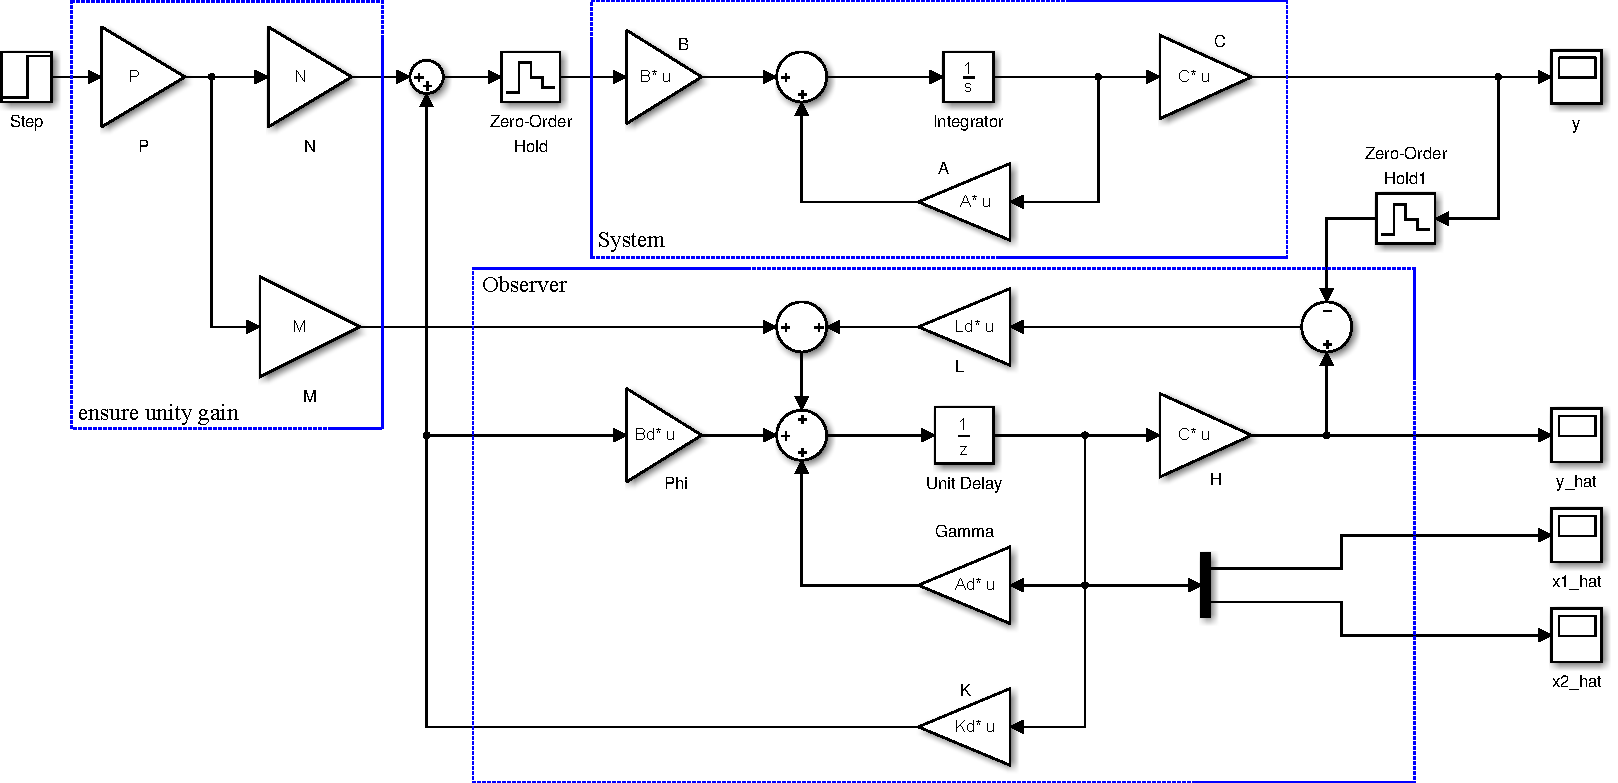
\includegraphics[scale=0.6]{observer_2_order.pdf}
	\caption{Simulink implementation of the discrete observer.}
	\label{fig:simulink_observer}
\end{figure}
The augmented (discrete) system with $\mathbf{x}_\text{augmented}\in\mathbb{R}^4$ is formulated as:
\begin{flalign*}
\begin{bmatrix}
\mathbf{x}(k+1) \\
\hat{\mathbf{x}}(k+1)
\end{bmatrix} &= \underbrace{\begin{bmatrix}
\boldsymbol\Gamma & \boldsymbol\Phi \mathbf{K}_d \\
-\mathbf{L}_d \mathbf{C} & \boldsymbol\Gamma + \boldsymbol\Phi \mathbf{K}_d + \mathbf{L}_d \mathbf{C} 
\end{bmatrix} }_{\boldsymbol\Gamma_{cl}}\begin{bmatrix}
\mathbf{x}(k) \\ \hat{\mathbf{x}}(k)
\end{bmatrix} + \underbrace{\begin{bmatrix}
\boldsymbol\Phi \mathbf{N} \\ \mathbf{M}
\end{bmatrix}}_{\boldsymbol\Phi_{cl}} x_\text{ref} \\
\mathbf{y}(k) &= \underbrace{\begin{bmatrix}
\mathbf{C} & 0 & 0
\end{bmatrix}}_{\mathbf{C}_{cl}}\begin{bmatrix}
\mathbf{x}(k) \\ \hat{\mathbf{x}}(k)
\end{bmatrix}
\end{flalign*}

\vspace{-3mm}
The discrete matrices $\boldsymbol\Gamma$ and $\boldsymbol\Phi$ can be found as \citep{bib:discrete_sampling}:
\begin{flalign}
\boldsymbol\Gamma &= \text{e}^{\mathbf{A}\, T_s} = \begin{bmatrix}
0.986 & 0.009 \\
-2.623 & 0.817
\end{bmatrix} \label{eq:Gamma_2}  \\
 \boldsymbol\Phi &= \int_0^{T_s}  \text{e}^{\mathbf{A}\, \mu} \, d \mu \cdot\mathbf{B} = \begin{bmatrix}
0.014 \\
2.623 
\end{bmatrix} \label{eq:Phi_2} 
\end{flalign}
\begin{tabular}{rl} 
where  &  \\
e& is the matrix exponential \\
$T_s$&  is the sampling time, $T_s=100\,$ms\\
\end{tabular}\\

The sampling time $T_s$ is according to Assistant Engineer Simon Jensen limited to 100\,Hz caused by the TCP/IP communication channel between ROS and the underlying hardware as seen in \autoref{fig:overview}.

The feedback matrix and  the observer gain can now be found. They will again be calculated in MATLAB, as the design procedure follow the exact same as in \autoref{sec:K_Nbar_1D_1storder}. The poles ($p_i$) will be placed from the below considerations:
\vspace{-3mm}
\begin{itemize}
	\itemsep-0.7mm
\item No overshoot in the closed loop step response, i.e. Im($p_i)=0$.
\item Asymptotic stability, i.e. $|p_i| < 1 $
\item Slow closed loop step response
\item Positive feedback, i.e. the controller and observer gains must be negative
\item An observer significantly faster than the closed loop system $\Gamma + \Phi \mathbf{K}_d$
\end{itemize}
\vspace{-7mm}
\begin{flalign}
\mathbf{K}_d &= -\texttt{acker}\left( \Gamma,\Phi,\begin{bmatrix}
0.5 & 0.35
\end{bmatrix} \right) = \begin{bmatrix}
 -11.360 & -0.305
 \end{bmatrix} \label{eq:Kd_2} \\
 \mathbf{L}_d &= -\texttt{acker}\left( \Gamma^T,\mathbf{C}^T,\begin{bmatrix}
0.01 & 0.02
\end{bmatrix} \right) = \begin{bmatrix}
  -1.773 \\
 -68.184
 \end{bmatrix} \label{eq:Ld_2}
\end{flalign}

\vspace{-5mm}
The matrix $\mathbf{M}$ introduces zeros in the closed loop transfer function  $\mathbf{y}(k)/x_\text{ref}$, which can be eliminated by designing the zeros close to the cut-off frequency. This means that the characteristic polynomial of the matrix $\Gamma_{za}+\tilde{\mathbf{M}}\mathbf{C}_{za}$ has zeros close to the cut-off frequency, where $\Gamma_{za}=\Gamma+\Phi \mathbf{K}_d + \mathbf{L}_d \mathbf{C}$ and $\mathbf{C}_{za}=-\mathbf{K}_d$ \citep{bib:Nbar}. The MATLAB function  \texttt{acker} can again be used:
\vspace{-2mm}
\begin{flalign*}
\tilde{\mathbf{M}} = - \texttt{acker}\left( \Gamma_{za}^T, \mathbf{C}_{za}^T, \begin{bmatrix}
0.01 & 0.02
\end{bmatrix} \right) = \begin{bmatrix}
  0.014 \\
   2.623
   \end{bmatrix}
\end{flalign*}

\vspace{-4mm}
To ensure unity gain between reference and system state, the $\mathbf{N}$ matrix can be computed as \citep{bib:Nbar}:
\vspace{-5mm}
\begin{flalign}
\mathbf{N} &= - \left( \mathbf{C}_{cl} \Gamma_{cl}^{-1} \tilde{\Phi}_{cl} \right)^{-1} \kk \text{where} \mm \tilde{\Phi} = \begin{bmatrix}
\Phi \\ \tilde{M}
\end{bmatrix} \nonumber \\
\mathbf{N} &= 13.739 \label{eq:N_2}
\end{flalign}

\vspace{-4mm}
The  matrix $\mathbf{M}$ ensuring unity gain between reference and observer state, can now be calculated as \citep{bib:Nbar}:
\vspace{-4mm}
\begin{flalign}
\mathbf{M} = \tilde{\mathbf{M}}\mathbf{N} = \begin{bmatrix}
 0.186 \\
  36.040
\end{bmatrix}
\label{eq:M_2}
\end{flalign}
\vspace{-0.2cm}
Thereby, all unknowns from \autoref{eq:observer} are calculated.

\begin{recap}[Control Law for Second Order Approximation]
	The complete controller based on the second order system approximation is now designed as:
\begin{flalign*}
&\textbf{1.}  \phantom{\mathbf{u}(k)}\hat{\mathbf{x}}(k+1) = \Gamma \hat{\mathbf{x}}(k) + \Phi \mathbf{K}_d \hat{\mathbf{x}}(k) + \mathbf{L}_d (\mathbf{C}\hat{\mathbf{x}}(k)-\mathbf{y}(k) ) + \mathbf{M} x_\text{ref} \\
&\textbf{2.} \phantom{\hat{\mathbf{x}}(k+1)}\mathbf{u}(k) = \sigma(\mathbf{x})k_0(\hat{\mathbf{x}})+(1-\sigma(\mathbf{x}))(\mathbf{N} \cdot x_\text{ref}-\mathbf{K}_d\hat{\mathbf{x}}(k))
\end{flalign*}
\begin{tabular}{rl} 
where  &  \\
$\sigma(\mathbf{x})$ & is computed from \autoref{eq:smoothness} with $\epsilon$ from in \ref{eq:epsilon_2} and the \gls{cbf} found in \ref{eq:cbf2}  \\
$k_0(\mathbf{x})$ & is computed from \autoref{eq:control_law} with Lie derivatives from \ref{eq:LgB_2} and \ref{eq:LfB_2}  \\
$\Gamma$ & is found in \autoref{eq:Gamma_2} \\
$\Phi$ & is found in \autoref{eq:Phi_2}  \\
$\mathbf{N}$ & is found in \autoref{eq:N_2}  \\
$\mathbf{M}$ & is found in \autoref{eq:M_2} \\
$\mathbf{L}_d$& is found in \autoref{eq:Ld_2} \\
$\mathbf{K}_d$ & is found in \autoref{eq:Kd_2} \\
$\mathbf{C}$ & is found in \autoref{eq:system:2}
\end{tabular}
\vspace*{-5mm}
\end{recap}
This completes the control design. The implementation constitutes both a MATLAB simulation and an actual implementation on the da Vinci robot in \gls{ros}. The MATLAB implementation is outlined first. 